
\graphicspath{{Chapters/03.DASH/img/}}

\section{Energy Consumption Due to ABR Streaming: An Experimental Analysis}
\label{sec:chap03:DASHinMobility}

Till now, we have analyzed the YouTube streaming system and the effect of the QUIC transport protocol on the different ABR algorithm. However, another factor exists when it comes to smartphone users. A large population watches the online video on their smartphones. In general, the smartphone runs on battery power, and among its users, a set of users watch online videos while they commute to and from work. During these times, most users do not have access to a power source to charge their smartphones.

So, while traveling, users mostly have to rely on cellular networks as WiFi hotspots are not available in the public commute most of the places. Due to the non-optimal placement of cellular base-station and massive crowds, it often lacks the desired signal quality, leading to higher battery drainage. To establish the cellular connectivity scenario, we have carried out an extensive measurement-based study for eleven months over five different cities in India, including urban areas as well as while travelling on highways. We have recorded the signal received by medium budget Moto G5 and Micromax phones, while using the cellular data connection of leading service providers in India, like Airtel, Reliance Jio, and Vodafone.


\begin{figure}[!h]
	\captionsetup[subfigure]{width=0.7\linewidth}
	\begin{center}
		\subfloat[\label{fig:chap03s3:technology_with_traj}Trajectory of a VoLTE-enabled android phone inside an academic campus. Associated network standards (4G, HDPA, UMTS, EDGE) highlighted using different colours)]{
			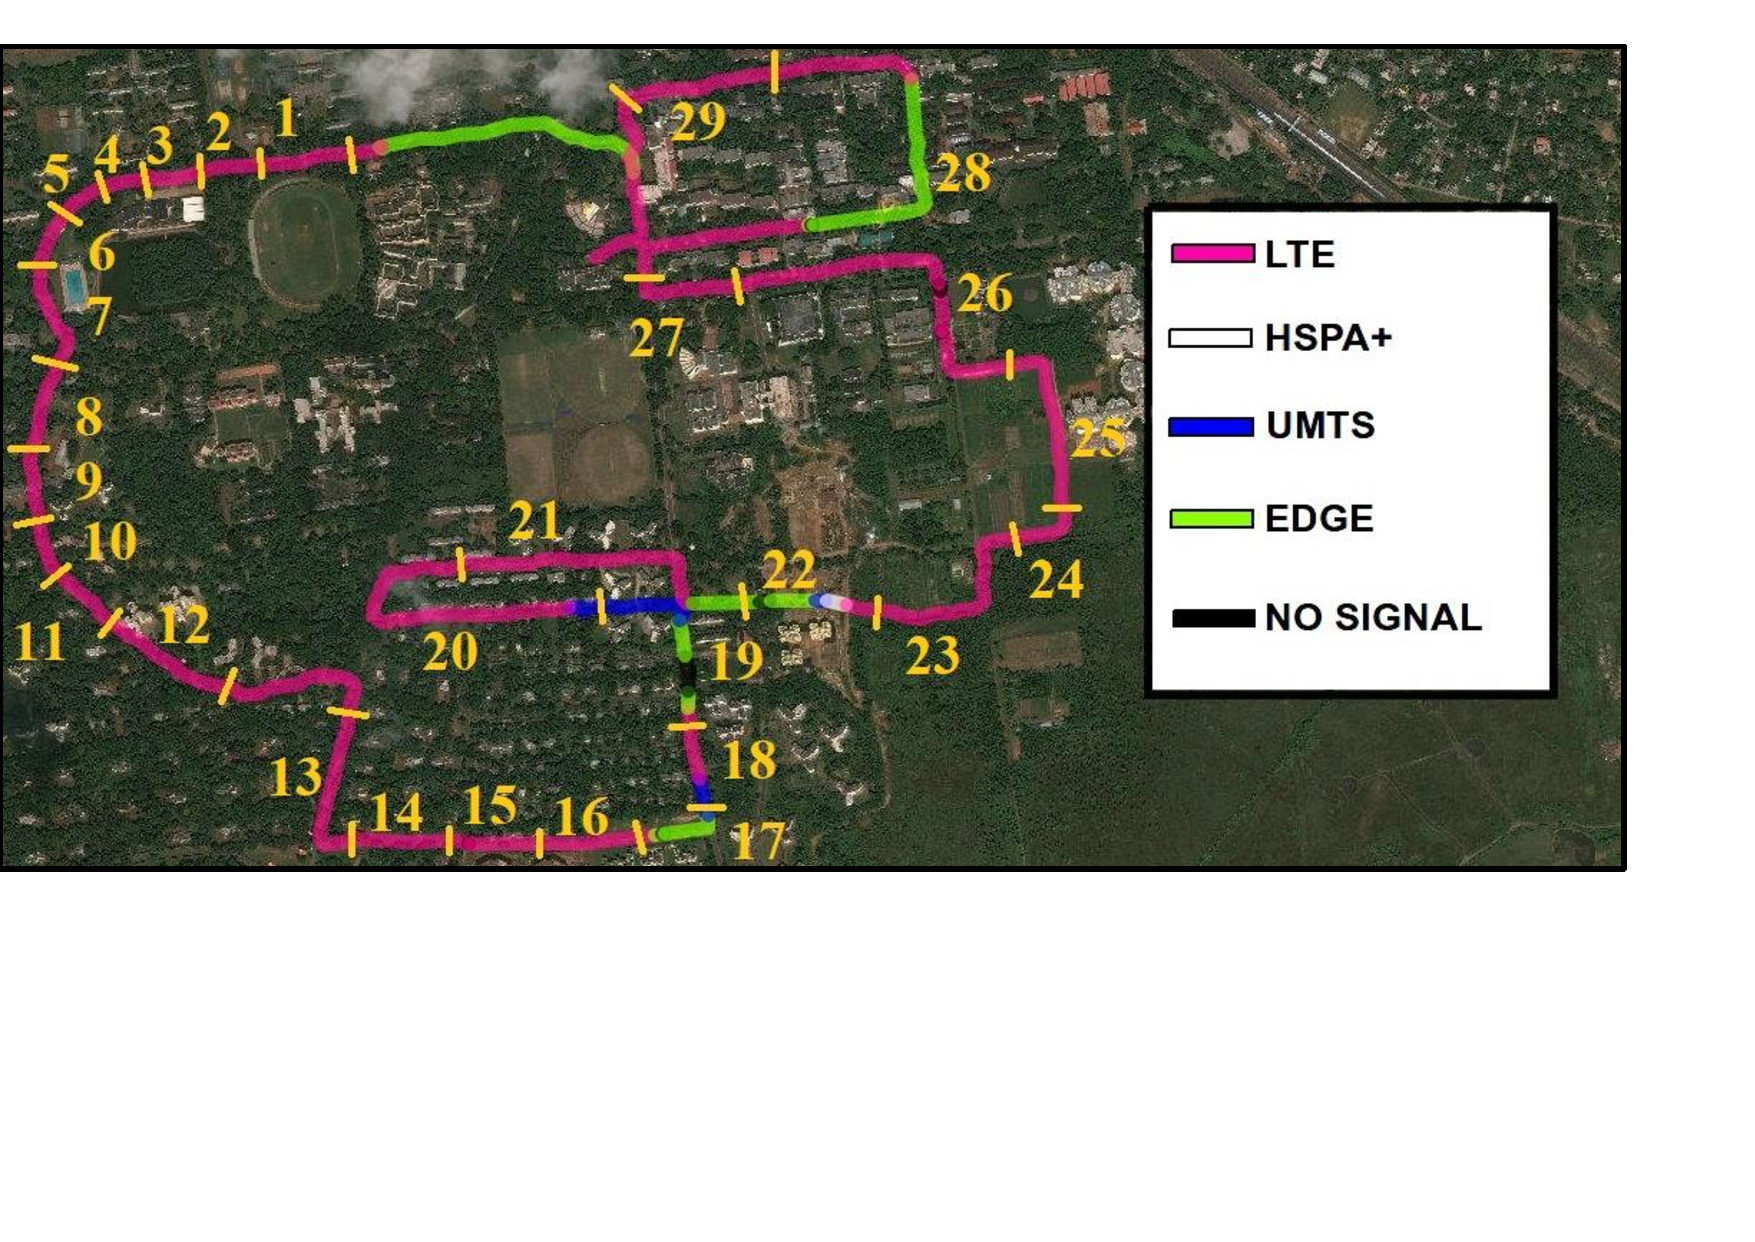
\includegraphics[width = 0.7\linewidth,trim={0cm 6cm 2cm 1cm}]{figures/traj.pdf}
		}\\
		\vspace{+5mm}
		\subfloat[\label{fig:chap03s3:pcap_RSSI}Packet trace of a 360p Youtube video download with the temporal variation in the \ac{RSSI} during the download]{
			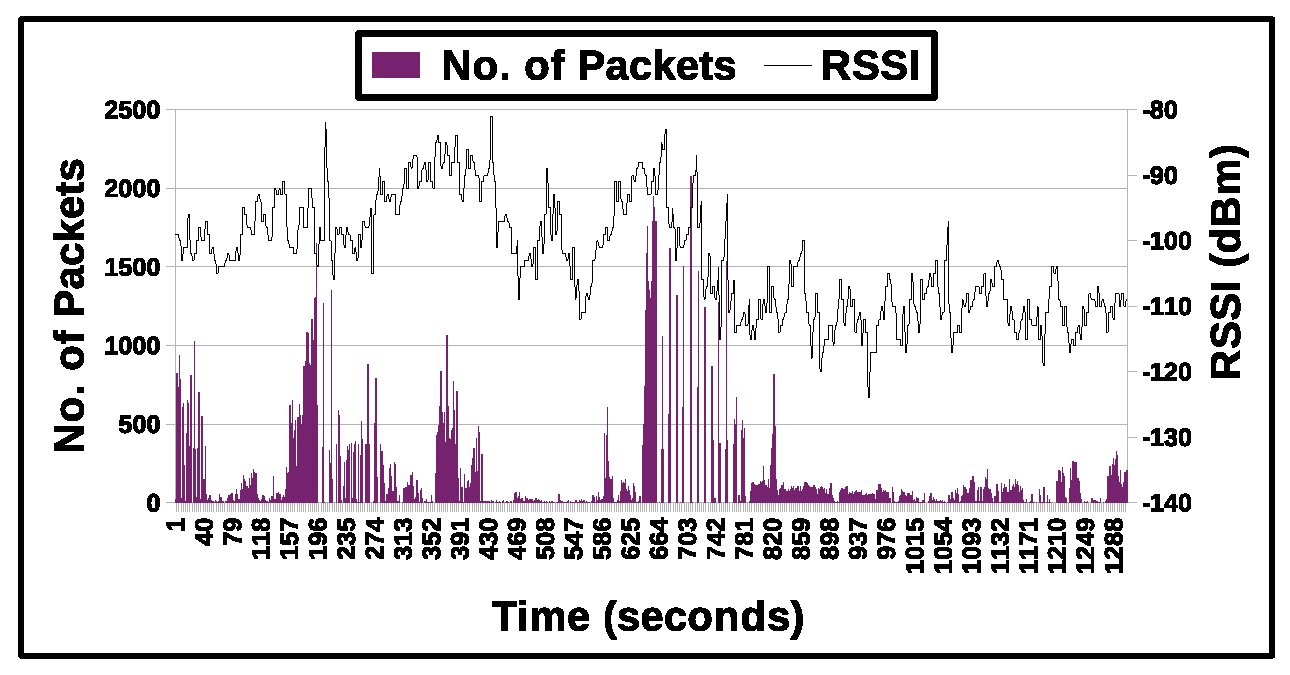
\includegraphics[width=0.7\linewidth,trim={0cm 0cm 0cm 1cm}]{figures/video_rssi_thrpt.eps}
		}
	\end{center}
	\caption{ Experimental Observations}
\end{figure}



A \textit{key finding} of this experiment is shown in \fig\ref{fig:chap03s3:technology_with_traj}, which displays the trajectory of a Moto G5 phone connected to the Airtel network on a single day over the IIT Kharagpur campus area of $8.5$ sq.km. It is seen that even within the small area covered, the phone connects to different generations of cellular technologies, each highlighted in different colours. Two inferences can readily be drawn from \fig\ref{fig:chap03s3:technology_with_traj}. (i) A service provider does not guarantee a complete \ac{4G} connectivity across the entire coverage region. A \ac{UE} often has to fallback to legacy \ac{3G} or \ac{2G} networks. (ii) Even when connected to \ac{4G}, the signal strength shows random variations. For example, for the experiments conducted, the \ac{RSSI} of \ac{4G} networks fluctuates between $-87$dBm to $-115$dBm. This portrays the typical connectivity scenario in many regions in India.
Another important observation from our experiments, shown in \fig\ref{fig:chap03s3:pcap_RSSI}, is that the volume of data downloaded by video players is not always commensurate with the current network signal strength. Several opportunities to download large chunks of data at high signal strength conditions remain unexploited.


In the previous experiment, we find that the cellular network condition is not consistent even over a small region. However, we want to know the relationship between various radio parameters such as signal strength, vertical and horizontal handover, device speed, etc., on the one hand, and throughput and energy consumption on the other hand. To develop this understanding, we have carried out an extensive measurement-based study, as discussed next.



\label{sec:chap03s3:EnDASHPilot}
\begin{figure}[!h]
	\captionsetup[subfigure]{width=0.49\linewidth}
	\begin{center}
		\subfloat[\label{fig:chap03s3:setup}The Experimental Setup inside a slow moving electric vehicle]{
			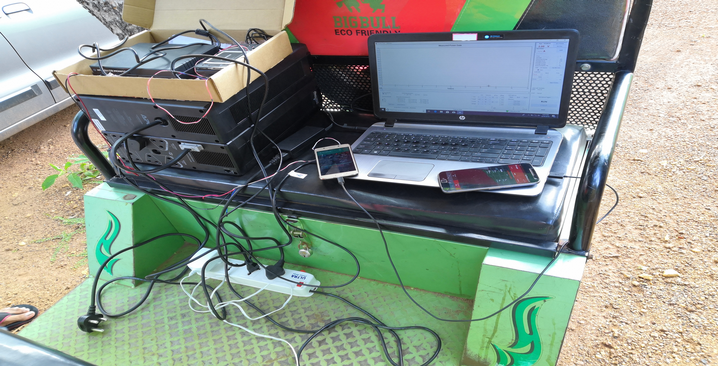
\includegraphics[width=0.49\linewidth]{figures/setup.png}
		}
		\subfloat[\label{fig:chap03s3:thptHO}Sorted throughput of the twenty-nine stretches of \fig{\ref{fig:chap03s3:technology_with_traj}} and its corresponding variations with RSSI, Vertical and Horizontal Handovers]{
			\fbox{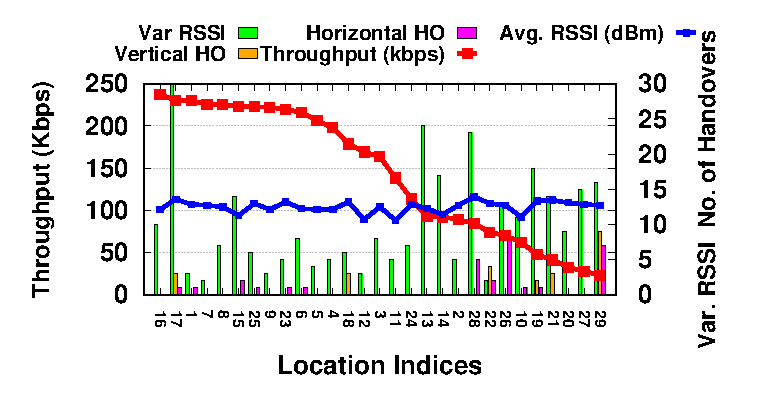
\includegraphics[width=0.49\linewidth]{new_results/pilot/location_throughput}}
		}\\
		\subfloat[\label{fig:chap03s3:powerHO}Variations of Power Consumption with RSSI, and Vertical and Horizontal Handovers over the user's trajectory shown in \fig{\ref{fig:chap03s3:technology_with_traj}}]{
			\fbox{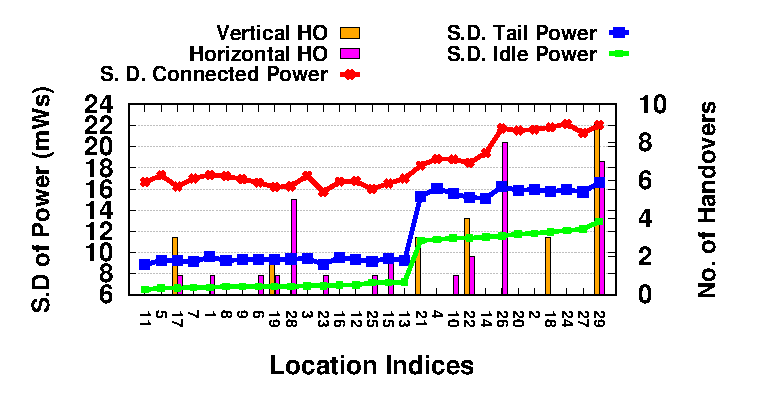
\includegraphics[width=0.49\linewidth]{new_results/pilot/location_power}}
		}
	\end{center}
	\caption{Experimental setup and Throughput and Power consumption variations of a user under mobility; Phone: Moto G5, Service Provider: Airtel}
\end{figure}

%\blue{
%To setup the context, we
%}

%To design an energy efficient video streaming algorithm, which tunes playback buffer length with cellular network throughput, we need a detailed comprehension of the complex relationships between radio related parameters, such as signal strength, vertical and horizontal handovers, speed, etc., on one hand, and throughput and energy consumption on the other hand. To develop this understanding, we have carried out an extensive measurement based study as discussed next.
\subsection{Experimental Set-up}
For power consumption and energy profiling, we have selected medium budget VoLTE enabled smartphones -  Moto G5  (\$149) and Micromax Canvas Infinity (\$87). \tbl\ref{tab:chap03s3:handset_details} outlines their configuration details. We record the power consumption of the phones using Monsoon Solutions High Voltage Power Monitor (HVPM) \cite{HVPM, Yang2018,Geng2015} (\fig\ref{fig:chap03s3:setup}) in both stationary and mobile conditions, when connected to three leading mobile internet service providers, Airtel, Reliance JIO, and Vodafone. The \ac{HVPM} records the power at a frequency of 5000 Hz. We have collected power consumption data in three different cities (Kolkata, Kharagpur, Guwahati).
\begin{table}[!h]
    \scriptsize
    \centering
      \caption{Details of the mobile handsets used}
    \begin{tabular}{|p{1cm}||p{6cm}|p{6cm}|}
    \hline
         \textbf{}  & \textbf{Moto G5 (Price: US\$ ~149)} & \textbf{Micromax Canvas Infinity (Price US\$ ~87)}\\
          \hline \hline
         N/W Tech. & GSM/ HSPA/ LTE &  GSM/ HSPA/ LTE\\ \hline
         N/W Speed & HSPA 42.2/5.76 Mbps, LTE Cat4 150/50 Mbps & HSPA 42.2/5.76 Mbps, LTE Cat4 150/50 Mbps\\ \hline
         OS & Android 7.0 (Nougat) & Android 7.1.2 (Nougat) \\ \hline
         Chipset & Qualcomm MSM8937 Snapdragon 430 (28 nm) & Qualcomm MSM8917 Snapdragon 425 (28 nm)\\ \hline
         CPU & Octa-core 1.4 GHz Cortex-A53 & Quad-core 1.4 GHz Cortex-A53\\ \hline
         GPU & Adreno 505 & Adreno 308\\ \hline
    \end{tabular}
    \label{tab:chap03s3:handset_details}
\end{table}

Besides power consumption, we have also collected extensive data on the observed throughput of mobile phones in public buses, cars, and while walking across five cities of India (Kharagpur, Kolkata, Guwahati, Bengaluru, Malda). This dataset also includes data collected while travelling on highways. We have used workloads of 6Mb, 100Mb, 1GB file download, as well as of video streaming using Netflix, Hotstar, SonyLiv and Amazon Prime. This has allowed a detailed energy profiling of the smartphones. The entire corpus of collected data traces amounts to more than 50GB and has been collected over a period of eleven months.

\subsection{Observations}
We next outline the observations from this experiment. We have considered two primary workloads- (a) file download, and (b) video streaming. \\
\begin{figure}[h]
    \centering
    \fbox{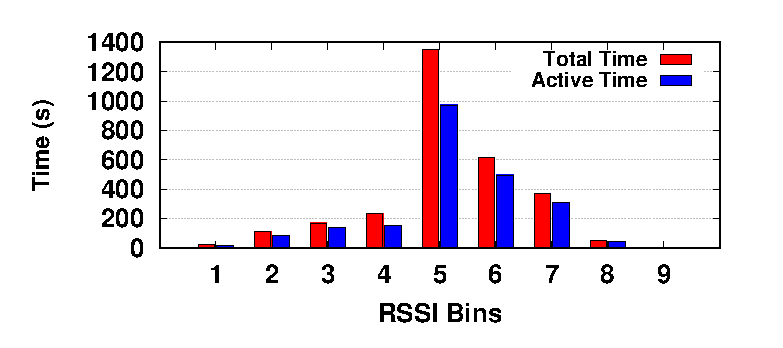
\includegraphics[width=0.7\textwidth]{new_results/pilot/rssi_bin_time}}
    \caption{Total time spent in each \ac{RSSI} bin and the active time in each bin}
    \label{fig:chap03s3:vid_time}
\end{figure}
\begin{figure}[h]
    \centering
    \fbox{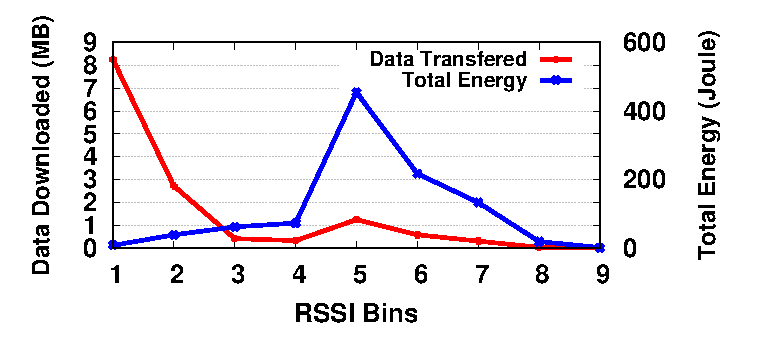
\includegraphics[width=0.7\textwidth]{new_results/pilot/rssi_bin_energy}}
    \caption{Amount of data downloaded \& Energy Consumption in \ac{RSSI} Bins}
    \label{fig:chap03s3:vid_thpt}
\end{figure}
% \begin{figure*}[t]%
% \centering
% \subfigure[Packet trace of a 360p Youtube video download with the temporal variation in the \ac{RSSI} during the download]{%
% \label{fig:pcap_RSSI}%
% 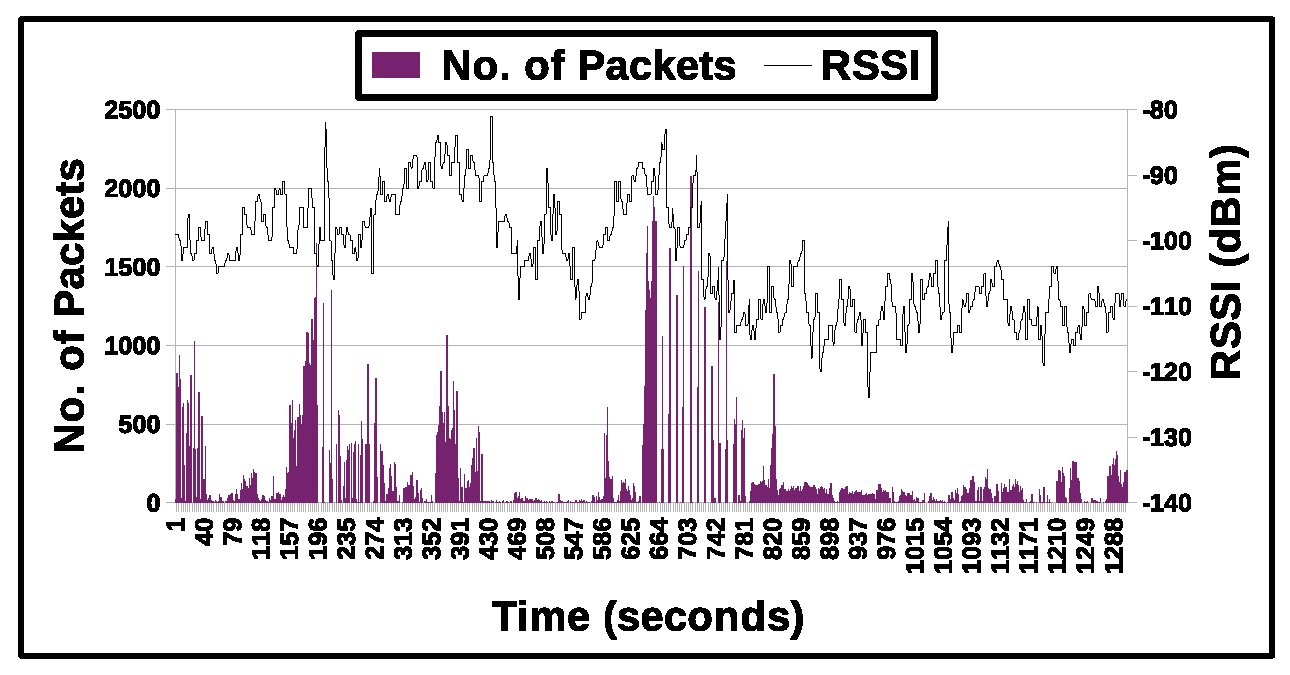
\includegraphics[width=0.31\textwidth]{figures/video_rssi_thrpt.eps}}%
% \hspace{0.1cm}
% \subfigure[Total time spent in each \ac{RSSI} bin and the active time in each bin]{%
% \label{fig:vid_time}%
% 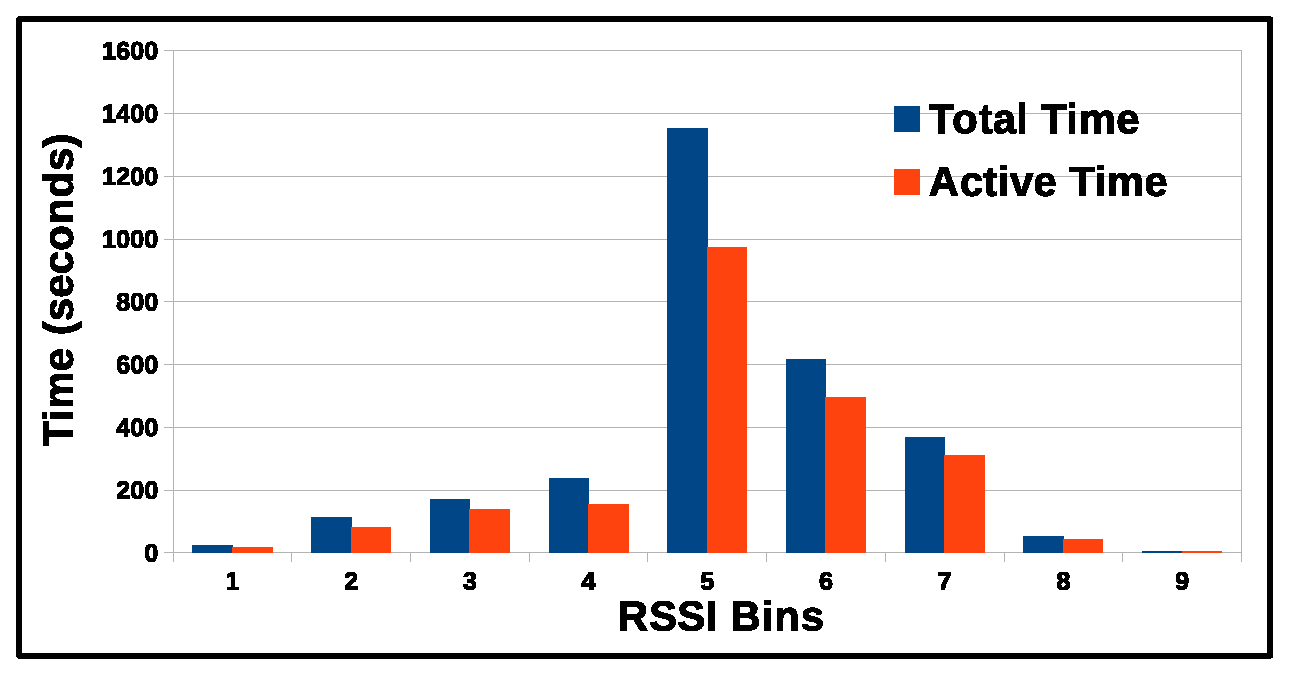
\includegraphics[width=0.31\textwidth]{figures/Video_Time_SNR_bins.eps}}%
% \hspace{0.1cm}
% \subfigure[Amount of data downloaded and Power Consumption in each \ac{RSSI} Bin]{%
% \label{fig:vid_thpt}%
% 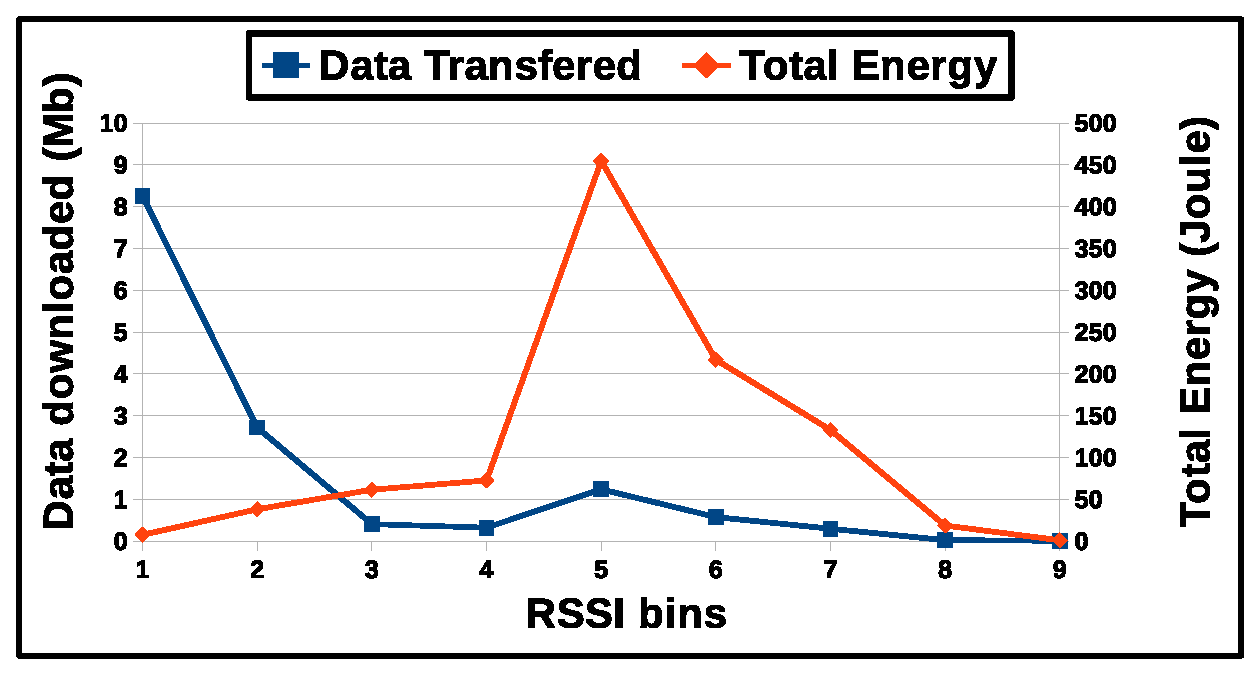
\includegraphics[width=0.31\textwidth]{figures/Video_thpt_power.eps}}%
% \caption{Statistics of YouTube video download to Moto G5 using Airtel mobile internet}\vspace*{-0.5cm}
% \end{figure*}
\subsubsection{File Download} We have used file downloads to profile the power consumption in different RRC states. To enable the download, we have developed  an HTTP client-server program, where the client program runs in the phone and the server  is hosted on a instance from Amazon Web Service (AWS). We have collected traffic traces, radio related information, and location and speed information using \ti{tcpdump}, Network Monitor Lite, and GPS Logger applications, respectively. The collected traffic traces have been analyzed using Wireshark. We have followed \cite{Yang2018} to derive  the RRC state diagram. Accordingly, to measure the \ti{IDLE} state power, we have kept the screen ON, uninstalled all non-default applications, kept all background applications disabled, the WiFi interface turned off, and the mobile network interface switched on but without any active traffic transmission. The corresponding power consumed by the operating system, processor, display, some default background and network-related operations, etc., constitutes the \ti{IDLE} state power.  We have continued measuring the power consumption starting from the \ti{IDLE} state, throughout the file download till the trace came back to the \ti{IDLE} power. Once a file download starts, a jump in power consumption is noted. After the download completes, it drops to an intermediate value during the tail time before returning to the \ti{IDLE} state \cite{Yang2018}. To derive the RRC states, we have downloaded files of different lengths several times using different phones and service providers in the different cities in stationary condition. The power consumption and dwell time of each RRC state has been found to be different for different phones, service providers as well as cities. With mobility, the average power consumed in each RRC state has remained the same  but the variance has increased.


\indent  Since the corpus of collected data traces is large, we use one such trace to discuss some interesting observations due to space limitations. We call this a `\ti{typical}' trace which was obtained on a single day when downloading 6MB files to the Moto G5 phone while moving around the IIT Kharagpur campus in a hybrid electric vehicle. The set-up is shown in \fig\ref{fig:chap03s3:setup}. As Airtel has significantly fluctuating signal quality inside the campus, we chose it as our service provider.  For this `\ti{typical}' trace we had downloaded a 6Mb file to our phone several times. During each download session, the vehicle had moved over a different stretch of the trajectory inside the IIT Kharagpur campus.  Of all the downloads, the twenty-nine stretches  shown in \fig{\ref{fig:chap03s3:technology_with_traj}} could be identified as valid. The sorted throughput over all the twenty-nine stretches of  \fig{\ref{fig:chap03s3:technology_with_traj}} is plotted in descending order in \fig{\ref{fig:chap03s3:thptHO}}. The $x$-axis represents the location indices corresponding to the sorted throughput. The mean and variance of the \ac{RSSI} and also the horizontal and vertical handovers in each of these stretches is shown in \fig{\ref{fig:chap03s3:thptHO}}.  It is observed that the throughput is affected more negatively by handovers than \ac{RSSI} fluctuations. For example, the average and the variance of \ac{RSSI} is nearly the same  in location stretches-\textbf{29} and \textbf{15}. However, stretch \textbf{29} has a lower throughput due to handovers. Again, vertical handovers between network technologies  are found to have a more negative impact on throughput than horizontal ones, as seen in location stretches {\bf 22}  and {\bf 4}.  The effect of handovers on the variation of \ti{CONNECTED}, \ti{TAIL} and \ti{IDLE} state power is shown in \fig\ref{fig:chap03s3:powerHO}. It is seen that stretches that witness handovers have a higher variance in  power consumption than no handover stretches. This is because, during handovers, there is a high amount of control information exchange which leads to the rise in \ti{IDLE} power. Moreover, handovers are associated with lower throughput which increases the \ti{CONNECTED} power. Fluctuating signal quality during handover increases the retransmissions and hence the TAIL state power variations.


$\mathrm{\mathbf{\underline{Takeaway:1}}}:$ \textit{The wireless network condition is best quantified by throughput which depends  significantly on phenomena such as handovers and not  on received signal quality alone.}

\subsubsection{Video Streaming}\label{sec:chap03s3:vstreaming}
To understand how throughput fluctuation affects video streaming,
we show the packet trace of a YouTube video of length 20 minutes captured when moving along the trajectory of \fig{\ref{fig:chap03s3:technology_with_traj}}.  Although we learn from the previous section that it is best to quantify the network condition using throughput, in this section we analyze the video download using \ac{RSSI} only. This is because it is difficult to capture the actual network throughput of a phone while any other application (in this case YouTube) is running.\\
\indent The  captured trace and the \ac{RSSI}  is shown in \fig{\ref{fig:chap03s3:pcap_RSSI}}. It is seen that the application downloads video chunks even at low \acp{RSSI}. To understand this, we have divided the \acp{RSSI} on the secondary $y$-axis of \fig{\ref{fig:chap03s3:pcap_RSSI}} into nine bins each of width five, starting from -81 dBm to -126 dBm. The time the \ac{UE} spends in each of these bins, and the time it remains active is given in \fig{\ref{fig:chap03s3:vid_time}}. It is seen that the percentage of time the \ac{UE} spends in the best \ac{RSSI} bin, i.e. \bin{1} (-85 to -81 dBm) is less than 1\%. In comparison, the highest dwell time   as well as the highest active time is recorded in \bin{5} where the \ac{RSSI} varies between -115 to -111 dBm. If we focus on the energy consumption in these \ac{RSSI} bins, as given in \fig{\ref{fig:chap03s3:vid_thpt}}, it is seen that the highest energy is also consumed by the phone in \ac{RSSI} \bin{5}. Another obvious effect of downloading at low signal strength is the low amount of data downloaded for a longer amount time; with reference to \ac{RSSI} \bin{5} in \fig{\ref{fig:chap03s3:vid_thpt}}.


\indent The rate at which the YouTube playback buffer is filled depends on: a) the bandwidth available, and b) the quality of the video requested by the user. Once the buffer length exceeds a threshold, the download stops and restarts only when the buffer length goes below the threshold. So, if the buffer is full when signal quality improves, then the phone does not download any video packet - a possible explanation for no data download between  430-547 seconds in \fig{\ref{fig:chap03s3:pcap_RSSI}}.


$\mathrm{\mathbf{\underline{Takeaway:2}}}:$ \textit{The current protocol of  video download attributes a higher weightage to the playback-buffer length than the user's instantaneous received signal strength or throughput, ensuing a significantly high energy consumption.}\\
%\indent The takeaways of the pilot study provide the design criteria for designing the EnDASH system, discussed next.
